\documentclass[fleqn]{llncs}
\usepackage[utf8]{inputenc}
\usepackage[bottom]{footmisc}
\usepackage{graphicx}
\usepackage{cite}
\usepackage{caption}
\usepackage{subcaption}
\captionsetup{compatibility=false}
%\usepackage{amsbsy}
\usepackage[fleqn]{amsmath}
\usepackage{booktabs}
\usepackage{breqn}
\usepackage{tikz}
\usetikzlibrary{arrows}
\usepackage{lipsum}
\usepackage[affil-it]{authblk}
\usepackage[english]{babel}
\interdisplaylinepenalty=2500
\pagenumbering{arabic}
\usepackage{array}
\usepackage[toc,page]{appendix}
\usepackage{bibnames}
\usepackage{tabto}
\usepackage{listings}

\title{Project 2 Clustering Report}
\author{Dong Xuanyu, Tiehang Duan, Yifu Yin}
\institute{Department of Computer Science and Engineering\\The State University of New York at Buffalo\\Buffalo, NY 14260, United States\\
\email{xuanyudo@buffalo.edu, yifuyin@buffalo.edu, tiehangd@buffalo.edu}}

\begin{document}

\maketitle

    \begin{abstract}
    This project implements clustering using three single thread and one Parallel algorithm. Single thread algorithms include k-means clustering, hierarchical agglomerative clustering with single link(min), and density based clustering. Parallel algorithm includes Map Reduce k-means clustering. Clustering is by definition, to find similar groups of data in a dataset, such that each group are similar to each other and different to others. Clustering is important in many fields. For example image processing, market research, data analysis and preprocess for other algorithms. \textbf{Python code with implementation is available on Github page: 
    \url{https://github.com/xuanyudo/Clustering-Project}.}
    \end{abstract}

\section{Model Description}
\subsection{K-Means}

K-Means clustering is an easy to implement, efficient and wildly used way to cluster data. Abstractly it is implemented in following steps:

1) Randomly initialize k centers.

2) Assign each data point to the closest center generated from previous step. Every points assigned to the same point is now a cluster.

3) For each cluster, calculate it's centroid. Move the center to the newly calculated centroid. 

4) Repeat Step 2 and Step 3 until clusters remain the same or centers remain the same.\\
The disadvantage of k-means includes sensitive to initialization, requirement of clusters count k, performs poorly under differing density, differing dataset size and irregular shape. There are ways to optimize initialization, but in this report we split data into k equal length clusters, and compute initial center from those clusters. 
    
\subsection{Hierarchical Agglomerative Clustering with Single Link(Minimal)}
Hierarchical Agglomerative Clustering is less efficient but no longer dependent on hyperparameter k. It is flexible and we are able to get any number of clusters by splitting down the hierarchy. In order to determine the structure of hierarchy, we need to determine the Inter-Cluster Distance function. Which includes min, max, average and centroid. In this project we are using min function. And abstractly it is implemented in following steps:

1). Set every single data point as cluster of singleton

2). For every clusters, find two clusters that contains closest data points, combine them together using two tree leaf nodes and set the their parent as the new cluster.

3) If there are more than two clusters left, repeat step 2.\\
Some advantage and disadvantage of Hierarchical Agglomerative Clustering is dependent on the Inter-Cluster Distance function, and in our case, it is good at finding clusters with arbitrary shapes, but it is sensitive to noises and outliers. 

\subsection{Density Based Clustering}
Density Based Clustering does not dependent on cluster number hyper-parameter k. It is insensitive to shape, size and outliers of the dataset. But it performs bad under varying density, and it is also sensitive to density hyper-parameter MinPts and eps. Abstractly it is implemented in following steps:

1). Find an undiscovered core point using MinPts. Which are points what have more or equal to MinPts points around it's radius range eps.

2). Find all core points within eps, add all discovered points within the range of eps of those points and add them into a new cluster.

3) If there are anymore undiscovered core point, repeat step 1.\\
Note that there is way to determine eps and MinPts by plotting sorted distance of every point to its kth nearest neighbor, but for this project, we are using MinPts = 4 and eps = 1.


\subsection{Map Reduce K-Mean}
Map-Reduce framework performs large scale distributed computing by separating the computational task into two separate steps: Map step and Reduce step. During the Map step, the model generate (key value) pairs, where the keys are the attributes that we want to aggregate and perform computation afterwards. Combiners can be involved in the map function to pre-process the data, where it aggregates the key value pairs on the current node, and can be seen as a local reducer. During the reducing step, data of the same key are aggregated onto the same reducer and perform computation accordingly. For the Map Reduce program tailored for the Kmeans algorithm, during the Map phase, we create pairs with centroid ID as the key and related features as the related value. Then during the reduce phase, the new coordinates are calculated for each of the centroid, which is straight forward after the data points belonging to each cluster have been aggregated together. 


\section{Model Implementation}
\subsection{Implementation of K-Means}
For the implementation of K-means, We have used K=5 for number of clusters. And we have implemented it similar to the pseudo code. For initialization, we split data into K random clusters with equal length and generate centers from those. And then for every genes, We compute the closest center calculated using euclidean distance and add the gene into that cluster. To calculate centers, we add every points together by dimension and divide by cluster length, Then we repeat until calculated centroid is same as previous centroid. We also provide options for initializing centroid which tester can set any K points to be the initial cluster center. In order to improve clustering result accuracy, we repeat k-mean algorithm N(num_iter) times and compute jaccard coefficients with our result and ground truth label. Lastly, we take the cluster result with highest jaccard coeffiecient value as our optimal k-mean result.


\subsection{Implementation of Hierarchical Agglomerative Clustering with Single Link(Minimal)}
(1) initialize all node itself as a cluster. Also every node has a target cluster initially to themselves. (2) we use euclidean distance to calculate distant between all node to others and put the distant in ascending order. (3) keep popping from the distant list and merge two clusters to one and set the target cluster of second one to the first and then delete the second cluster. (4) Based on our K value, we stop step (3) until there are only K number of cluster.

\subsection{Implementation of Density Based Clustering}
For density based clustering, we can two parameters which are search range(ep) and minimum numbers of point need to be explored(min\_supp). (1) iterating through all node to find out all core, border and outlier node by counting nodes explored (if ${>=}$min\_supp then core, if 0 then outlier, otherwise border). (2) iterating through all core point, for each of core point initializes a cluster with core point in it and add all explored points into a queue and cluster and keep popping out the node from the queue and marks it as explored point, if the node is core point, add all sub_node explored by that point, keep above process until all node marked as explored. (3) if the node is a outlier, we put it into a separate list for visualization purpose.

\subsection{Implementation of Map Reduce Clustering}
For the main program, it feeds in three parameters which are input data file, initialized centroids which are done by randomized selection, and the output file path. Then in the main class, we iteratively call the mapper function and reducer function until the result converges. Hash maps are used to store the aggregated (Centroid ID: [data points]) pairs so as to make the access speed faster. Before launching the map and reduce jobs, we call new configuration() which specifies the appropriate interfaces and abstract classes. The job client then submits the job and configuration to the JobTracker which then assumes the responsibility of distributing the configuration to the slaves, which is initialized through new Job(conf,"KMeans"). The setting of the job is done through a series of methods defined under the Job class which includes: setJarByClass, setMapperClass, setReducerClass, setOutputKeyClass, setOutputValueClass, etc. 




\section{Experiment Result}


For Data visualization, we are using PCA algorithm from sklearn.decomposition package. And as you see, the resulting graph includes one huge cluster and is hard to visually separate into clusters. And for performance of each algorithm, we use Jaccard's coefficient to determine.

\subsection{Result K-Means}


\begin{figure}
	\centering
	\begin{subfigure}{0.45\textwidth}
		\centering
        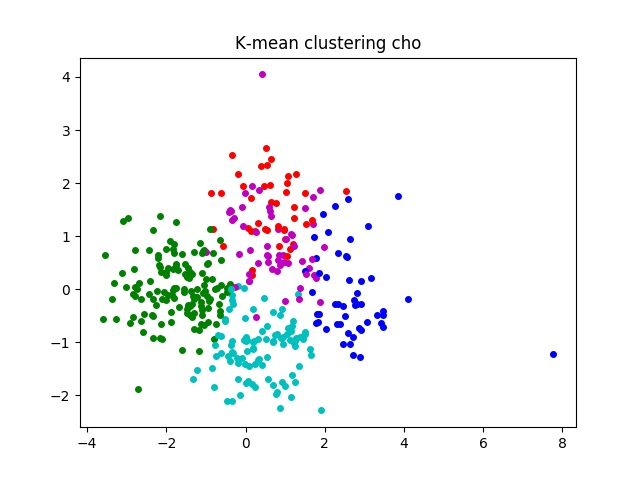
\includegraphics[width=\textwidth]{k_meancho.jpg}
		\caption{}
        \label{Fig9_1}
	\end{subfigure}
	\begin{subfigure}{0.45\textwidth}
		\centering
	    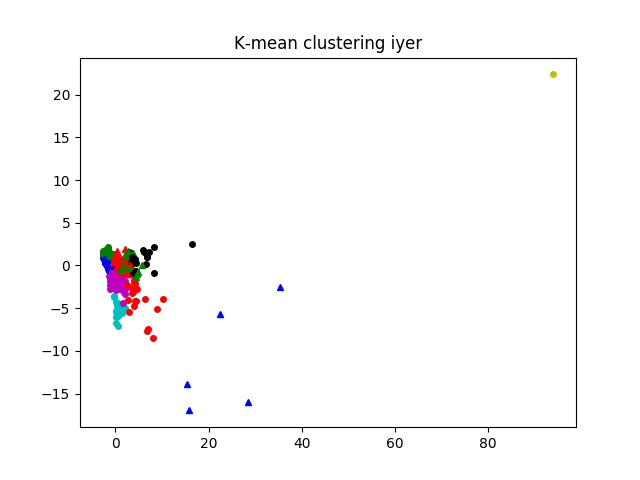
\includegraphics[width=\textwidth]{k_meaniyer.jpg}
	    \caption{}
	    \label{Fig9_2}
    \end{subfigure}
\caption{}
\label{fig9}
\end{figure}


As you see from Fig.1, According to nature of K-means, namely poor performance toward cluster of different sizes and different density, K-means algorithm had separated the big cluster into K cluster of similar size, and split the denser cluster toward the left side into two clusters. From the graph we can conclude k-means does not perform well in this situation.

\subsection{Result Hierarchical Agglomerative Clustering with Single Link(min)}




\begin{figure}
	\centering
	\begin{subfigure}{0.45\textwidth}
		\centering
		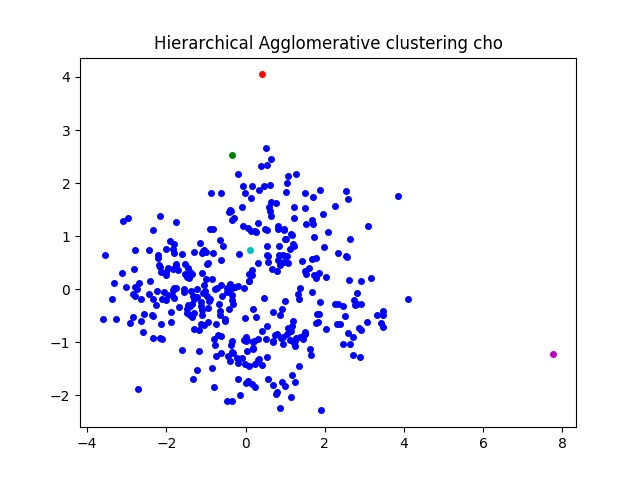
\includegraphics[width=\textwidth]{hiercho.jpg}
		\caption{}
		\label{Fig10_1}
	\end{subfigure}
	\begin{subfigure}{0.45\textwidth}
		\centering
		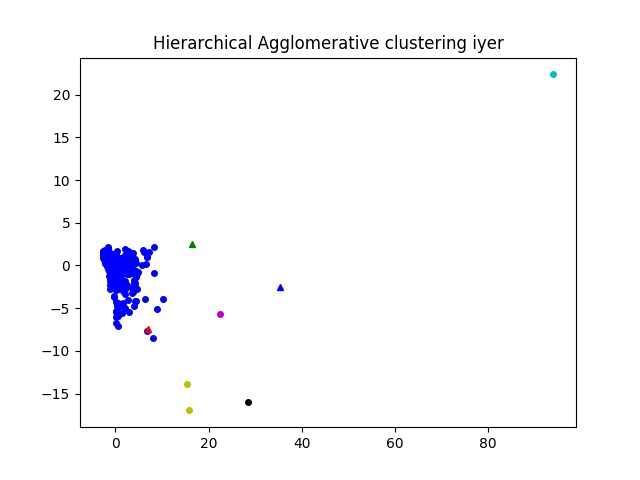
\includegraphics[width=\textwidth]{hieriyer.jpg}
		\caption{}
		\label{Fig10_2}
	\end{subfigure}
	\caption{}
	\label{fig10}
\end{figure}




As you see from result in Fig.1, Due to Inter-Cluster Distance function min being sensitive to outliers and noises, those points that located far away from center cluster put into it's own cluster. And the big cluster is kept as one cluster

\subsection{Result of Density Based}


\begin{figure}
	\centering
	\begin{subfigure}{0.45\textwidth}
		\centering
		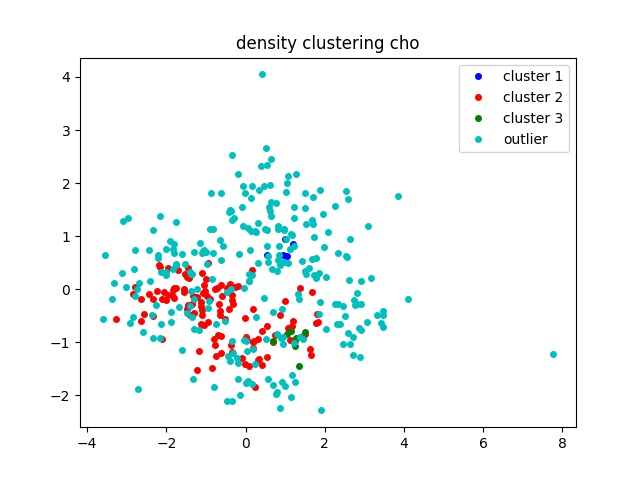
\includegraphics[width=\textwidth]{densitycho.jpg}
		\caption{}
		\label{Fig11_1}
	\end{subfigure}
	\begin{subfigure}{0.45\textwidth}
		\centering
		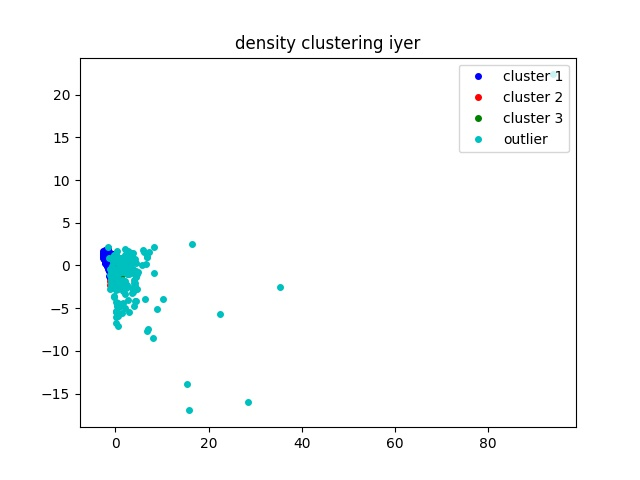
\includegraphics[width=\textwidth]{densityiyer.jpg}
		\caption{}
		\label{Fig11_2}
	\end{subfigure}
	\caption{}
	\label{fig11}
\end{figure}





Due to high amount of minimum point need to be explored by node, there exist lots of outlier nodes. Because density based clustering perform badly with dataset contains varying density, that's why it performs bad in cho.txt which doesn't contains any outlier. however it performs slightly better than hierarchical clustering result after tuning the minsupp and search range in iyer.txt because density based clustering can explore outlier.

\begin{figure}
	\centering
	\begin{subfigure}{1\textwidth}
		\centering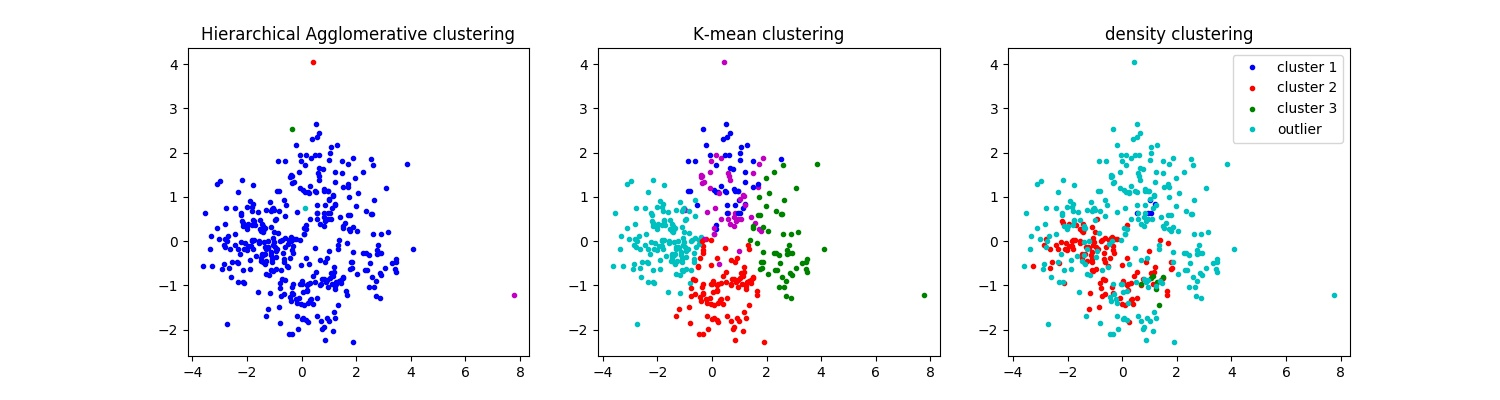
\includegraphics[width=1\textwidth]{all_three.jpg}
		\caption{Hierarchical Agglomerative, K-Means and Density Based Algorithm}
	\end{subfigure}
	\caption{(a) Hierarchical Agglomerative clustering result visualization of cho.txt, (b) K-Means clustering result visualization of cho.txt, (c) Density Based clustering result visualization of cho.txt.}
	\label{fig2}
\end{figure}
\begin{figure}
	\centering
	\begin{subfigure}{1\textwidth}
		\centering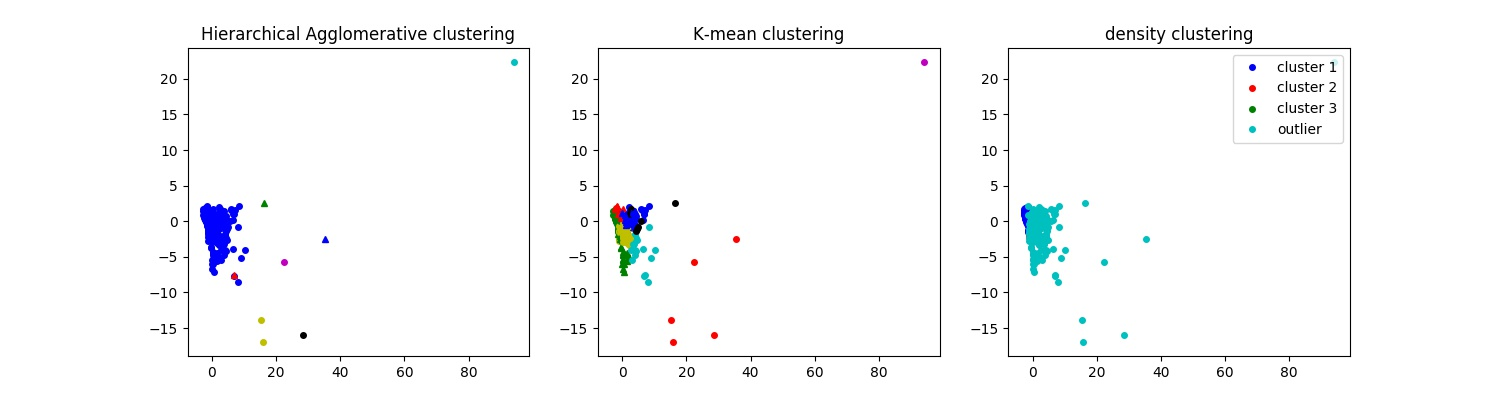
\includegraphics[width=1\textwidth]{all_threeiyer.jpg}
		\caption{Hierarchical Agglomerative, K-Means and Density Based Algorithm}
	\end{subfigure}
	\caption{(a) Hierarchical Agglomerative clustering result visualization of iyer.txt, (b) K-Means clustering result visualization of iyer.txt, (c) Density Based clustering result visualization of iyer.txt.}
	\label{fig3}
\end{figure}
Jaccard-coefficients of cho.txt:\\
Kmean: 0.4100590299936184\\ 
Hierchical: 0.22839497757358454\\
Density: 0.20433377280653256\\

Jaccard-coefficients of iyer.txt:\\
Kmean: 0.4265362385770463\\ 
Hierarchical: 0.15824309696642858\\
Density: 0.28350284799805836\\

As you can see Kmean algorithm gives the best clustering result for these two dataset. Density based clustering perform well on dataset contains outliers. Hierarchical clustering is sensitive to noise and 
outlier, which gives the worrest performance.

\subsection{Result of Map Reduce Clustering}

We run the implementation of Map Reduce Kmeans method on the cho.txt and iyer.txt dataset provided in the project. When the number of clusters is initialized to be the same as ground truth number, the result is shown in Figure \ref . We can see the clustering result is the same as what we got in the previous section for normal Kmeans implementation. It takes the program  seconds to complete the computation for cho.txt and  seconds for iyer.txt. We calculated both the random index and Jacob coefficient. For cho.txt, the program is getting 0.7849 on Rand Index and 0.3417 on Jaccard Coefficient, for iyer.txt, the program is getting 0.7837 on Rand Index and 0.2793 on Jaccard Coefficient. For normal Kmeans implemented in the previous section, we are getting 0.8085 for Rand Index on cho.txt and 0.7890 for Rand Index on iyer.txt, we can see the result that we achieve here is similar (especially given that for normal Kmeans implementation, we are doing 10 runs and picking the best performance out).

\begin{figure}
	\centering
	\begin{subfigure}{0.45\textwidth}
		\centering
		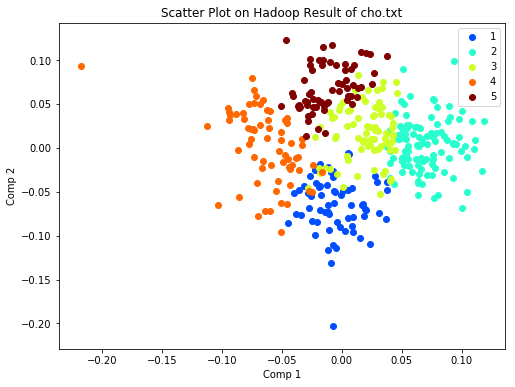
\includegraphics[width=\textwidth]{hadoop_scatter_cho.png}
		\caption{}
		\label{Fig12_1}
	\end{subfigure}
	\begin{subfigure}{0.45\textwidth}
		\centering
		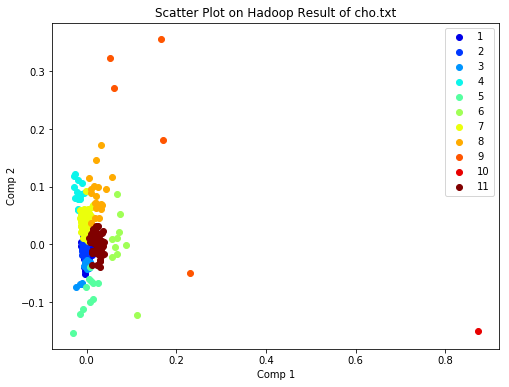
\includegraphics[width=\textwidth]{hadoop_scatter_iyer.png}
		\caption{}
		\label{Fig12_2}
	\end{subfigure}
	\caption{}
	\label{fig12}
\end{figure}

\end{document}
